\section{Formulación del problema}
¿Cómo se pueden enseñar y fortalecer las habilidades de “aprender a aprender” y de “escucha activa” en los estudiantes de ingeniería de sistemas de la Universidad del Valle, sede Tuluá?


\section{Descripción del problema}
El avance tecnológico está reconfigurando el panorama laboral actual, planteando desafíos significativos para la estabilidad y el futuro profesional de muchos trabajadores, en especial aquellos que realizan tareas rutinarias que pueden ser automatizadas y que carecen de habilidades blandas. Es más, investigaciones realizadas por la Universidad de Harvard, la Fundación Carnegie y el Centro de Investigación de Stanford encontraron que el 85\% del éxito profesional proviene de tener habilidades blandas bien desarrolladas y habilidades interpersonales. Las habilidades duras, que incluyen habilidades técnicas y conocimientos, solo representan el 15\% del éxito profesional \cite{NationalSoftSkills2024}.
\\
\\
Sin embargo, a pesar del reconocimiento de la importancia de las habilidades blandas, existe discrepancia entre las demandas del mercado laboral y la formación que se recibe en la universidad para el trabajo. De acuerdo a un reporte del 2019 \cite{Wilkie2019}, the Society for Human Resource Management descubrió que el 51\% de sus miembros que participaron en una encuesta contestaron que los sistemas educativos han hecho poco o nada para ayudarles a abordar la escasez de estas habilidades, en especial el pensamiento crítico; la innovación y creatividad; la capacidad para lidiar con la complejidad y la ambigüedad; y la comunicación.
\\
\\
The Accreditation Board of Engineering (ABET) \cite{ABET2021} considera crucial para evaluar la calidad de la educación en ingeniería, la preparación que los estudiantes reciben para la práctica. Como resultados esperados para los estudiantes la ABET establece que deben tener habilidades no técnicas o habilidades blandas como la capacidad de aprender a aprender, la escucha activa y el conocimiento del contexto social, político, económico y global de su trabajo, así como el impacto de su trabajo en estos contextos.
\\
\\
Los programas de educación superior de ingeniería de sistemas no incorporan del todo las habilidades blandas en su estrategia de enseñanza-aprendizaje, ni proporcionan una concientización reiterada acerca de la importancia y las consecuencias de las deficiencias de estas \cite{hernandez2020}. En la Universidad del Valle, sede Tuluá, la formación académica de sus ingenieros es enfática en lo técnico y teórico, generando una desconexión con la realidad del mundo laboral moderno y los factores decisivos para la obtención de un primer empleo y un éxito profesional. La figura 1 (árbol de problemas), identifica las causas y efectos de la falta de desarrollo de habilidades blandas en los ingenieros de sistemas de la Universidad del Valle, sede Tuluá.

\begin{figure}[ht!]
    \centering
    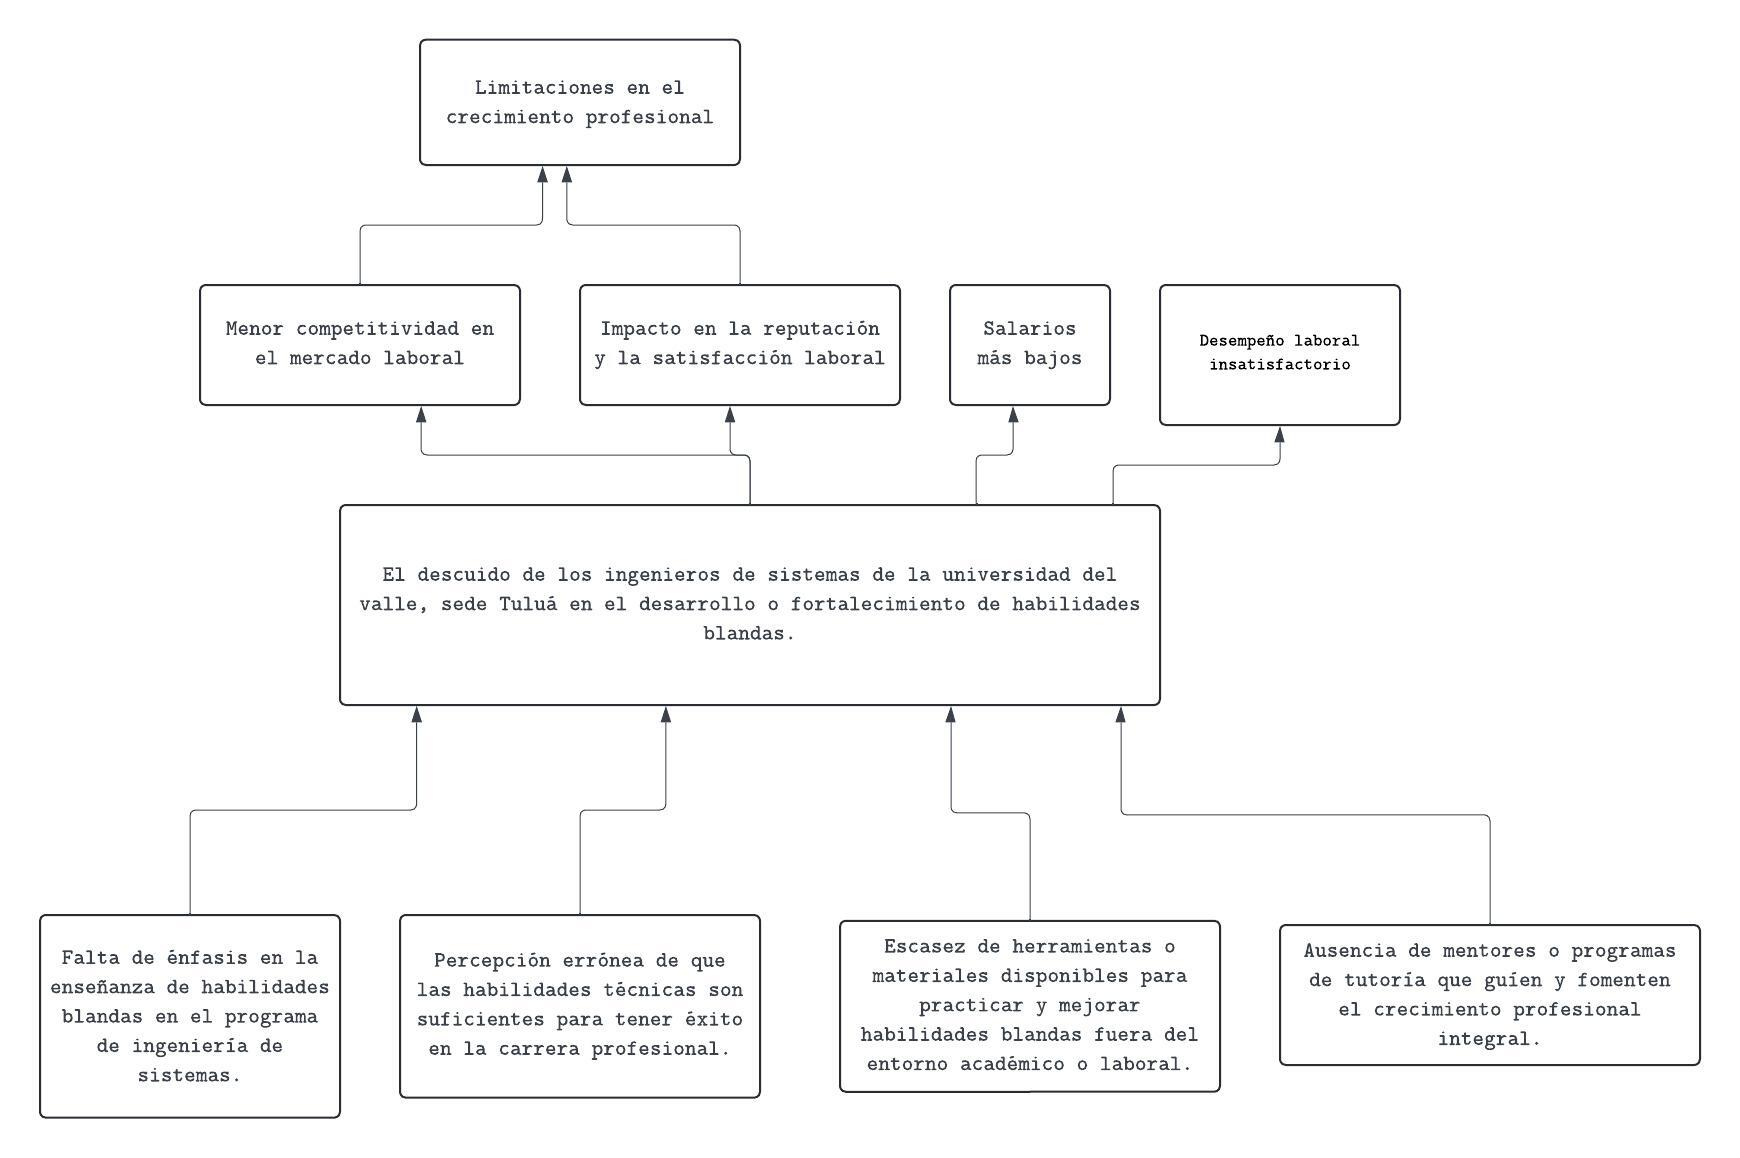
\includegraphics[width=\textwidth]{Figuras/Árbol de problemas.jpeg}
    \caption{Árbol de problemas. Elaboración propia.}
    \label{fig:problema_formulacion}
\end{figure}
\newpage